\section{Soviet Early Lead: Sputnik and Vostok}

\subsection{Sputnik and the shock in America}
In Soviet Early Lead: Sputnik and Vostok, Sputnik and the shock in America shows how the superpowers turned ballistic missile research into a public contest for orbital and lunar firsts. Leaders on both sides treated each launch as proof of industrial capacity, scientific maturity, and ideological confidence. \cite{siddiqi2010} \cite{logsdon2010}

The section Sputnik and the shock in America highlights engineers such as Sergei Korolev and Wernher von Braun, whose teams adapted military rockets for exploration. Reliability, telemetry, and life-support constraints turned each mission into a chain of irreversible decisions under extreme time pressure. \cite{siddiqi2010} \cite{logsdon2010}

For Sputnik and the shock in America, historians compare Soviet secrecy with NASA's televised milestones. Public audiences learned mission jargon, followed countdowns, and debated whether moonshots justified their cost while terrestrial crises continued. \cite{siddiqi2010} \cite{logsdon2010}

Additional detail on Sputnik and the shock in America: archives now reveal how failures were hidden, retried, or reframed. The Moon Race was never a smooth arc; it was a sequence of gambles where a single explosion could shift budgets and national narratives overnight. \cite{siddiqi2010} \cite{logsdon2010}

In Soviet Early Lead: Sputnik and Vostok, Sputnik and the shock in America shows how the superpowers turned ballistic missile research into a public contest for orbital and lunar firsts. Leaders on both sides treated each launch as proof of industrial capacity, scientific maturity, and ideological confidence. \cite{siddiqi2010} \cite{logsdon2010}

The section Sputnik and the shock in America highlights engineers such as Sergei Korolev and Wernher von Braun, whose teams adapted military rockets for exploration. Reliability, telemetry, and life-support constraints turned each mission into a chain of irreversible decisions under extreme time pressure. \cite{siddiqi2010} \cite{logsdon2010}

For Sputnik and the shock in America, historians compare Soviet secrecy with NASA's televised milestones. Public audiences learned mission jargon, followed countdowns, and debated whether moonshots justified their cost while terrestrial crises continued. \cite{siddiqi2010} \cite{logsdon2010}

Additional detail on Sputnik and the shock in America: archives now reveal how failures were hidden, retried, or reframed. The Moon Race was never a smooth arc; it was a sequence of gambles where a single explosion could shift budgets and national narratives overnight. \cite{siddiqi2010} \cite{logsdon2010}

In Soviet Early Lead: Sputnik and Vostok, Sputnik and the shock in America shows how the superpowers turned ballistic missile research into a public contest for orbital and lunar firsts. Leaders on both sides treated each launch as proof of industrial capacity, scientific maturity, and ideological confidence. \cite{siddiqi2010} \cite{logsdon2010}

The section Sputnik and the shock in America highlights engineers such as Sergei Korolev and Wernher von Braun, whose teams adapted military rockets for exploration. Reliability, telemetry, and life-support constraints turned each mission into a chain of irreversible decisions under extreme time pressure. \cite{siddiqi2010} \cite{logsdon2010}

For Sputnik and the shock in America, historians compare Soviet secrecy with NASA's televised milestones. Public audiences learned mission jargon, followed countdowns, and debated whether moonshots justified their cost while terrestrial crises continued. \cite{siddiqi2010} \cite{logsdon2010}

Additional detail on Sputnik and the shock in America: archives now reveal how failures were hidden, retried, or reframed. The Moon Race was never a smooth arc; it was a sequence of gambles where a single explosion could shift budgets and national narratives overnight. \cite{siddiqi2010} \cite{logsdon2010}

In Soviet Early Lead: Sputnik and Vostok, Sputnik and the shock in America shows how the superpowers turned ballistic missile research into a public contest for orbital and lunar firsts. Leaders on both sides treated each launch as proof of industrial capacity, scientific maturity, and ideological confidence. \cite{siddiqi2010} \cite{logsdon2010}

The section Sputnik and the shock in America highlights engineers such as Sergei Korolev and Wernher von Braun, whose teams adapted military rockets for exploration. Reliability, telemetry, and life-support constraints turned each mission into a chain of irreversible decisions under extreme time pressure. \cite{siddiqi2010} \cite{logsdon2010}

\subsection{First human in space: Yuri Gagarin}
In Soviet Early Lead: Sputnik and Vostok, First human in space: Yuri Gagarin shows how the superpowers turned ballistic missile research into a public contest for orbital and lunar firsts. Leaders on both sides treated each launch as proof of industrial capacity, scientific maturity, and ideological confidence. \cite{siddiqi2010} \cite{logsdon2010}

The section First human in space: Yuri Gagarin highlights engineers such as Sergei Korolev and Wernher von Braun, whose teams adapted military rockets for exploration. Reliability, telemetry, and life-support constraints turned each mission into a chain of irreversible decisions under extreme time pressure. \cite{siddiqi2010} \cite{logsdon2010}

For First human in space: Yuri Gagarin, historians compare Soviet secrecy with NASA's televised milestones. Public audiences learned mission jargon, followed countdowns, and debated whether moonshots justified their cost while terrestrial crises continued. \cite{siddiqi2010} \cite{logsdon2010}

Additional detail on First human in space: Yuri Gagarin: archives now reveal how failures were hidden, retried, or reframed. The Moon Race was never a smooth arc; it was a sequence of gambles where a single explosion could shift budgets and national narratives overnight. \cite{siddiqi2010} \cite{logsdon2010}

In Soviet Early Lead: Sputnik and Vostok, First human in space: Yuri Gagarin shows how the superpowers turned ballistic missile research into a public contest for orbital and lunar firsts. Leaders on both sides treated each launch as proof of industrial capacity, scientific maturity, and ideological confidence. \cite{siddiqi2010} \cite{logsdon2010}

The section First human in space: Yuri Gagarin highlights engineers such as Sergei Korolev and Wernher von Braun, whose teams adapted military rockets for exploration. Reliability, telemetry, and life-support constraints turned each mission into a chain of irreversible decisions under extreme time pressure. \cite{siddiqi2010} \cite{logsdon2010}

For First human in space: Yuri Gagarin, historians compare Soviet secrecy with NASA's televised milestones. Public audiences learned mission jargon, followed countdowns, and debated whether moonshots justified their cost while terrestrial crises continued. \cite{siddiqi2010} \cite{logsdon2010}

Additional detail on First human in space: Yuri Gagarin: archives now reveal how failures were hidden, retried, or reframed. The Moon Race was never a smooth arc; it was a sequence of gambles where a single explosion could shift budgets and national narratives overnight. \cite{siddiqi2010} \cite{logsdon2010}

In Soviet Early Lead: Sputnik and Vostok, First human in space: Yuri Gagarin shows how the superpowers turned ballistic missile research into a public contest for orbital and lunar firsts. Leaders on both sides treated each launch as proof of industrial capacity, scientific maturity, and ideological confidence. \cite{siddiqi2010} \cite{logsdon2010}

The section First human in space: Yuri Gagarin highlights engineers such as Sergei Korolev and Wernher von Braun, whose teams adapted military rockets for exploration. Reliability, telemetry, and life-support constraints turned each mission into a chain of irreversible decisions under extreme time pressure. \cite{siddiqi2010} \cite{logsdon2010}

For First human in space: Yuri Gagarin, historians compare Soviet secrecy with NASA's televised milestones. Public audiences learned mission jargon, followed countdowns, and debated whether moonshots justified their cost while terrestrial crises continued. \cite{siddiqi2010} \cite{logsdon2010}

Additional detail on First human in space: Yuri Gagarin: archives now reveal how failures were hidden, retried, or reframed. The Moon Race was never a smooth arc; it was a sequence of gambles where a single explosion could shift budgets and national narratives overnight. \cite{siddiqi2010} \cite{logsdon2010}

In Soviet Early Lead: Sputnik and Vostok, First human in space: Yuri Gagarin shows how the superpowers turned ballistic missile research into a public contest for orbital and lunar firsts. Leaders on both sides treated each launch as proof of industrial capacity, scientific maturity, and ideological confidence. \cite{siddiqi2010} \cite{logsdon2010}

The section First human in space: Yuri Gagarin highlights engineers such as Sergei Korolev and Wernher von Braun, whose teams adapted military rockets for exploration. Reliability, telemetry, and life-support constraints turned each mission into a chain of irreversible decisions under extreme time pressure. \cite{siddiqi2010} \cite{logsdon2010}

\begin{figure}[htbp]
\centering
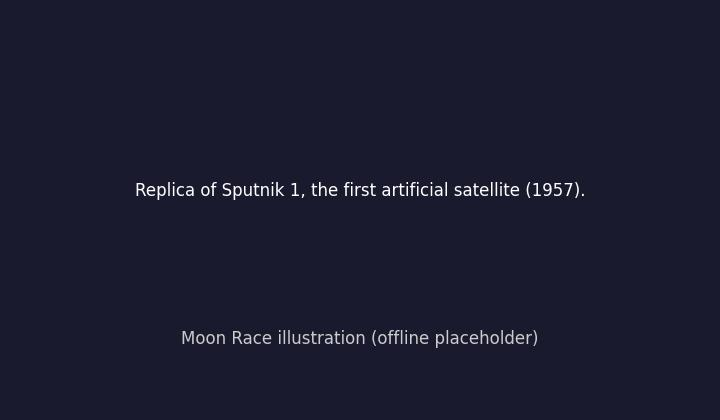
\includegraphics[width=0.88\linewidth]{figures/ch02_sputnik.jpg}
\caption{Replica of Sputnik 1, the first artificial satellite (1957).}
\label{fig:ch_replica_of_sputnik_1_the_first_a}
\end{figure}

\clearpage
\begin{otherlanguage}{hebrew}
\subsection*{סיכום הפרק}

פרק זה עוסק ביתרון הסובייטי המוקדם עם השקת לוויין ראשון והטסת האדם הראשון לחלל. הישגים אלו הזעזעו את ארצות הברית והאיצו את תגובתה.

\end{otherlanguage}
